\chapter{Background}
\label{chap:background}

In questo capitolo affronteremo i concetti base necessari alla comprensione del funzionamento dei protocolli quantistici di distribuzione delle chiavi, degli attacchi che possono essere portati a termine contro tali protocolli e dei meccanismi di difesa.

\section{Principi e teoremi di base}
\label{sec:principi_teoremi}
Di seguito si mostrano i principi e teoremi essenziali allo scopo della comprensione dei protocolli di QKD.

\subsection{Principio di Heisenberg}
Uno dei principi fondamentali della fisica quantistica è il principio di indeterminazione di Heisenberg (PIH). Esso afferma che, in meccanica quantistica, solo una proprietà di una coppia di proprietà coniugate può essere misurata con precisione arbitraria. Con il termine astratto "proprietà" si indicano, ad esempio, la posizione e il momento di una particella. È dunque impossibile conoscere con precisione il momento data una misura precisa della posizione e viceversa. Quanto detto è riassunto dalla seguente formula:
$$ \Delta x \cdot \Delta p_x \geq \frac{\hbar}{2} $$
$\Delta x$ è l'incertezza sulla misura della posizione e $\Delta p_x$ è l'incertezza sulla quantità di moto, mentre $\hbar$  è la costante di Plank ridotta, pari a $6.582 \times 10^{-16} eV \cdot s$. È facile osservare come per ottenere una misurazione precisa di $x$ (i.e. $\Delta x$ piccolo) sia necessaria una elevatissima imprecisione nella misurazione di $p_X$ (i.e. $\Delta p_x$ grande).

\subsection{Teorema "no cloning"}
Una conseguenza di PIH è il teorema "no cloning", che sottolinea l'impossibilità di creare copie identiche di un stato quantico (ad esempio momento e posizione) arbitrario. Infatti, si potrebbe pensare che sia possibile aggirare il principio di incertezza generando duplicati di uno stato quantico, così da misurare una differente proprietà coniugata per ogni copia. Tuttavia, tentare di copiare, dunque "leggere" lo stato di una particella, comporta modificare le proprietà della stessa e, di conseguenza, verrebbe a generarsi un duplicato diverso dall'originale. 

\section{Quantum entanglement}
Dicasi quantum entanglement il legame che si forma tra due particelle tali che, quando una particolare proprietà viene misurata nella prima, lo stato opposto viene rilevato istantaneamente nella corrispondente particella correlata, detta "entangled". Questo è vero indipendentemente dalla distanza delle due particelle (\textit{action at distance}); tuttavia, risulta impossibile predire a priori (prima di una misurazione) quale stato verrà osservato. Di conseguenza, è impossibile comunicare sfruttando il quantum entanglement senza un'operazione preliminare nel canale classico che dia indicazioni ad un ricevente su come effettuare la misurazione degli stati quantistici inviati.  

\section{Concetti di base sui protocolli di QKD}
Il modello di base di un generico protocollo di QKD (si veda la figura \ref{fig:qkd_diagram_and_trusted_center}) coinvolge tipicamente due parti, riferite come Alice (sender) e Bob (receiver), le quali vogliono accedere al canale di comunicazione al fine di scambiarsi informazioni in modo sicuro. Esiste inoltre un terzo ente, detto Eve (abbreviazione di eavesdropper), che si assume avere accesso al canale ed essere dotato di risorse quantistiche arbitrarie. In riferimento alla sezione \ref{sec:principi_teoremi}, il canale di comunicazione quantistico è la fibra ottica, la particella corrisponde al fotone. 
\begin{figure}[h]
    \centering
    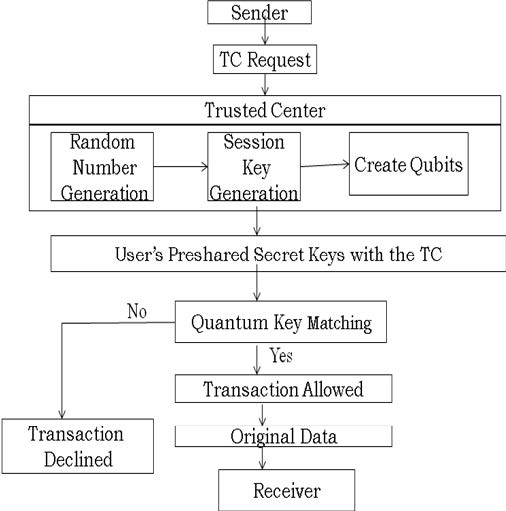
\includegraphics[width=11cm]{qkd_diagram_and_trusted_center}
    \caption{Architettura di un protocollo di QKD \cite{security_qkdp}.}
    \label{fig:qkd_diagram_and_trusted_center}
\end{figure}

Nel corso della trattazione ci focalizzeremo su protocolli a chiave privata, detti anche a chiave condivisa: questa permette di cifrare il contenuto informativo che si desidera scambiare tra le due parti così da garantire \textit{confidentiality}, ossia che eventuali malintenzionati, seppur capaci di intercettare i messaggi, non siano in grado di interpretarli. Alice e Bob conservano una copia della medesima chiave, ossia una stringa alfanumerica generata secondo i dettami del protocollo. Il problema fondamentale risulta proprio la condivisione della chiave: di ciò si occupano i protocolli di QKD.
In alcuni di questi, gli utenti ottengono la chiave segreta tramite un terzo ente, detto trusted center (TC), presentato nell'articolo \cite{security_qkdp} e di cui si riporta nella figura (\ref{fig:qkd_diagram_and_trusted_center}). Dal momento che tre parti sono coinvolte nella negoziazione della chiave di sessione, i corrispondenti protocolli sono detti three-party key distribution protocol. In caso vi siano solamente Alice e Bob, le mansioni del TC sono assorbite dalle due parti. \\
Le comunicazioni tra Alice e Bob avvengono mediante invio e ricezione di fotoni, opportunamente polarizzati a seconda che debbano rappresentare uno 0 o un 1 binario: tale polarizzazione è rappresentata da una combinazione lineare di stati quantistici di una base, ossia un insieme di stati tra loro ortogonali. Alcuni esempi di basi saranno illustrati nel capitolo \ref{chap:protocolli_qkd}.
Il TC ed i partecipanti sincronizzano la base di polarizzazione attraverso una chiave segreta precondivisa. Durante la distribuzione della seconda chiave, quella di sessione, la chiave precondivisa viene combinata con una stringa random per produrre una terza chiave, che sarà utilizzata per cifrare quella di sessione. Ciò garantisce che Bob non riceva lo stesso messaggio cifrato anche a parità di chiave di sessione, poiché la stringa random varia ad ogni trasmissione. La struttura delle chiavi dipende dal protocollo in uso.

Il qubit - quantum bit - è l'unità informativa di base della comunicazione attraverso canali quantistici. Similmente al bit classico, può codificare due stati che sono determinati dalle caratteristiche fisiche della particella che rappresenta l'unità informativa. Lo stato quantistico di un qubit viene determinato, come già indicato, mediante la combinazione lineare degli stati quantistici di una base. Le basi sono determinate dai protocolli di QKD.

\section{Vulnerabilità e attacchi ai protocolli di QKD}
Come già indicato, l'idea di base dei protocolli di QKD è che Alice e Bob comunichino per mezzo di fotoni che, se opportunamente polarizzati, rappresentano la codifica di precisi bit individuati dalle due parti della comunicazione

Il PIH permette di garantire che Eve non possa misurare questi fotoni ed inoltrarli a Bob senza che ne venga alterato lo stato, perciò senza che Eve riveli la propria presenza. Dunque i protocolli di QKD possono considerarsi incondizionatamente sicuri, nel senso che se anche Eve disponesse di capacità computazionali e tempo illimitato, non riuscirebbe a scardinare la sicurezza di tali protocolli per via del fatto che essa di base sulle leggi della fisica.

Nonostante ciò, i protocolli considerati sono suscettibili agli attacchi man-in-the-middle (MitM), in cui l'eavesdropper si finge Bob nei confronti di Alice e viceversa, simultaneamente. Tale attacco risulta implausibile da prevenire, a meno di una mutua autenticazione preventiva tra le due parti. Per di più, non è immediato comprendere se la sicurezza incondizionata sia rispettabile anche in presenza di rumore o di strumentazione imperfetta (ad esempio, circuiti di generazione della chiave condivisa mal progettati).

\subsection{Denial of Service}
L'attacco Denial of Service (DoS) è una tipologia di cyber-attacco in cui l'attaccante mira a rendere i servizi offerti da un dispositivo (o da una rete di dispositivi) non disponibili. Nei canali classici, questo avviene saturando le risorse o la banda. Per quanto concerne le comunicazioni previste dai protocolli di QKD, si ha una terza opzione: è sufficiente che Eve vada a misurare le particelle in transito nel canale per alterarne lo stato e dunque impossibilitarne la corretta lettura a Bob. Risulta perciò infattibile schermarsi completamente da un attacco di questo tipo, a meno di poter impedire la presenza dell'attaccante lungo il canale di comunicazione. In alternativa, \cite{ddos_mitigation_sdn} dimostra che è possibile, se si dispone di fibre ottiche multi-core, passare a un secondo canale appena Eve viene rilevato.

\subsection{Photon Number Splitting}
Emettere singole particelle, nella maggior parte dei casi fotoni, rende vulnerabili ad attacchi di tipo Photon Number Splitting (PNS), descritto per la prima volta da Brassard et al. in \cite{limitation_practical_qc}. L'attacco prevede che Eve prelevi una porzione dei fotoni in transito da Alice verso Bob durante tutta la durata della loro comunicazione.\\
Posto che sia Bob che Alice siano a conoscenza dell'inaffidabilità del canale trasmissivo e delle possibili perdite di informazioni, Eve può impedire il passaggio di parte del flusso di fotoni diretto verso Bob facendogli credere che questo fenomeno sia dovuto interamente alla natura del canale. In questo modo, Eve può celare la propria presenza alle parti coinvolte nella comunicazione. \\
Al fine di contrastare PNS, l'articolo \cite{revealing_pns} spiega come sia possibile rilevare la distribuzione dei fotoni nel canale e il tempo di trasmissione, permettendo di confrontarli con i valori attesi per aumentare la capacità di identificare la presenza dell'attaccante.

\subsection{Intercept-resend}
L'obiettivo di Eve è ottenere, almeno in parte, la chiave condivisa tra Alice e Bob. La strategia più immediata è intercettare i qubit in transito da Alice a Bob: tuttavia, questi non possono essere banalmente copiati, in quanto ciò contraddirebbe il teorema "no-cloning". Dunque, per estrarre il contenuto informativo, l'\textit{eavesdropper} Eve è forzato alla lettura (quindi alla distruzione dell'informazione) delle particelle. La misurazione di queste ultime prevede però la scelta casuale di una base, come si vedrà nel capitolo \ref{chap:protocolli_qkd}: se questa scelta si rivela inesatta (cioè viene scelta una base diversa da quella utilizzata da Alice), allora il successivo rinvio delle particelle verso Bob, codificate con la nuova base, lo porterà ad effettuare misurazioni dall'esito completamente casuale.

\subsection{Beam splitting}
Dal momento che utilizzare sorgenti a singolo fotone nelle comunicazioni quantistiche tra Alice e Bob espone ad attacchi di tipo PNS e non garantisce la ricezione dei fotoni da parte di Bob, si è pensato di inviare flussi di fotoni per mezzo di impulsi laser. Tuttavia, l'impiego di impulsi apre la strada ad attacchi Beam Splitting \cite{beam_splitting}, ossia alla possibilità da parte di un \textit{eavesdropper} di "trafugare" parte dei fotoni nell'impulso in transito. Solitamente un attacco di questo tipo garantisce a Eve di acquisire informazioni sui bit scambiati e, al tempo stesso, di celare la propria presenza dal momento che Bob vedrebbe giungere comunque a destinazione parte dell'impulso originale e penserebbe che la componente persa sia dovuta alle inevitabili perdite del canale trasmissivo. \\
In presenza di lunghi canali di trasmissione l'attacco risulta difficilmente realizzabile per via del fatto che le perdite di segnale sarebbero elevate a prescindere dall'intervento di Eve e quindi un'eccessiva riduzione del segnale ricevuto da Bob farebbe nascere in lui il sospetto della presenza di un attaccante.\\
\cite{trusted_noise} afferma di aver realizzato un meccanismo di difesa che consente di rilevare la presenza di un \textit{eavesdropper} anche in presenza di un canale estremamente rumoroso. Il concetto si basa su misurazioni statistiche del rumore previsto all'interno del canale e delle perdite attese di segnale: se queste superano una data soglia, calcolate statisticamente, allora viene notificata la presenza di un \textit{eavesdropper}.


\subsection{Physical side-channels}
Date le limitazioni degli attacchi che sfruttano il canale in fibra ottica, al fine di dischiudere il contenuto informativo tra Alice e Bob è possibile sfruttare mezzi trasmissivi alternativi come radiazioni elettromagnetiche, dissipazione del calore, rumore acustico, registrazione dei tempi computazionali o dei consumi energetici. Ad esempio, si rileva il tempo impiegato dal dispositivo per produrre la chiave di sessione, così da poterla ricavare. 
Allo stato dell'arte odierno, sia che si parli di protocolli classici di \textit{key exchange} che di QKD, non esiste una soluzione ufficiale in grado di far fronte in via permanente a questo attacco.

\subsection{Disturbi nella comunicazione come sintomo di eavesdropping}
Nei sistemi reali, se Alice e Bob scoprono che le loro misurazioni non sono correttamente correlate risulta arduo determinare se la discrepanza sia dovuta al canale trasmissivo rumoroso, alla strumentazione difettosa oppure alla presenza di un \textit{eavesdropper} che genera delle perturbazioni nei fotoni, misurandoli. Si assume dunque la presenza dell'attaccante e che quest'ultimo sia in possesso di informazioni sulla chiave condivisa da Alice e Bob al termine di un protocollo di QKD. Per questo motivo, i protocolli di QKD possono includere come ultimo passo dell'algoritmo una tecnica nota come \textit{privacy amplification} \cite{security_individual_realistic_qkd} che mira a ridurre l'informazione che Eve ha riguardo la chiave condivisa.  La tecnica prevede che venga fornito in ingresso a una funzione di hash scelta casualmente una stringa casuale di bit della stessa lunghezza della chiave condivisa. L'output della funzione risulta poi essere una stringa binaria (la nuova chiave condivisa) di lunghezza fissata e minore della lunghezza della chiave condivisa. La nuova chiave è più corta di quella originale di una quantità che varia in base a quanta informazione si stima essere in possesso dell'attaccante. Tali calcoli sono possibili misurando la discrepanza tra i bit letti da Bob rispetto a quelli intesi da Alice. La \textit{privacy amplification} garantisce che la probabilità che l'attaccante possegga informazioni riguardo la nuova chiave sia molto bassa.